% Manuscript v4 (after review round 2; see paper/REVIEW_round2.md and paper/RESPONSE_round2.md).
% v3 (before the round-2 review): manuscript_v3_before_round2_review.tex; v2: manuscript_v2_before_round2.tex.
% Target: Energy and Buildings (Elsevier, elsarticle). Earlier versions: manuscript_v1_before_review.tex (as reviewed),
% manuscript_v1_after_hybrid.tex (identical content). The hybrid dry cooler study moved to paper/hybrid/manuscript_hybrid.tex (review M1).
% Compile: pdflatex manuscript && bibtex manuscript && pdflatex manuscript && pdflatex manuscript (or Overleaf).
\documentclass[preprint,12pt,authoryear]{elsarticle}
\usepackage{amsmath,amssymb,graphicx,booktabs,siunitx,hyperref,xcolor}
\newcommand{\tbd}[1]{\textcolor{red}{[#1]}}
\graphicspath{{../results/figures/}}
\journal{Energy and Buildings}

\begin{document}
\begin{frontmatter}
\title{Cooling tower evaporation models in building energy simulation: a verified multi-method EnergyPlus framework
and its implications for data center water use}

\author{Liang Zhang}
\address{Department of Civil and Architectural Engineering and Mechanics, University of Arizona, Tucson, AZ, USA \tbd{confirm affiliation}}

\begin{abstract}
Building energy simulation is increasingly used to estimate data-center water use, but it computes cooling tower
evaporation with simplified relations. We present an open EnergyPlus Python-plugin framework that evaluates eight
evaporation models, from rules of thumb to the full Poppe model with supersaturated air, at the same
simulated operating point every timestep, with blowdown from makeup-water chemistry. The Poppe implementation agrees with
an independent solution within 0.01\,\%; on 126 measured fill tests it predicts the
outlet-air temperature within 0.84\,K rms, against 1.10\,K for a saturated-exit analysis, though evaporation was
not measured. For a fixed counterflow tower at full load, saturated-exit methods differ from Poppe by $-$19 to +11\,\%
across ambient conditions and empirical methods by $-$39 to +117\,\%. For a 1\,MW water-cooled data center in 14 climates,
the EnergyPlus default (saturated exit) gives 3.7--9.3\,\% less annual evaporation than Poppe (3.5--7.6\,\% excluding
liquid mist). With an ordinary fill meeting the same condenser-water temperature the shortfall persists at cool sites
(3--9\,\%), whereas at hot--dry sites the difference spans $-$2 to +11\,\%, its sign set by the tower's air-to-water ratio. Loss-factor estimates over their documented range (0.15--0.27\,\%/K) deviate by $-$22 to +122\,\%.
Under sourced treatment limits, and excluding the model's cycle bounds, each site's own makeup water changes makeup by
$-$16 to +44\,\% relative to the customary four cycles, so the cycles assumption matters as much as the evaporation model. We also show that the EnergyPlus \texttt{LossFactor} input is applied as a fraction rather than
a percentage.
\end{abstract}

\begin{highlights}
\item Eight tower evaporation models evaluated on the same EnergyPlus operating point
\item Poppe fits 126 measured fill tests better than saturated-exit analysis
\item EnergyPlus default gives 3.7--9.3\,\% less evaporation than Poppe in 14 climates
\item In hot--dry climates the sign of the difference depends on the tower's L/G
\item EnergyPlus applies its LossFactor input as a fraction, not a percentage
\end{highlights}

\begin{keyword}
Cooling tower \sep Evaporation \sep Poppe method \sep EnergyPlus \sep Data center \sep Water usage effectiveness
\end{keyword}
\end{frontmatter}

\section*{Nomenclature}
\begin{tabular}{ll}
$B$, $D_r$ & blowdown, drift [kg/s] \\
$c_{pa}, c_{pv}, c_{pw}$ & specific heat of dry air, vapour, liquid water [J/(kg\,K)] \\
$\mathcal{D}$ & denominator of the Poppe equations, Eq.~(2) [J/kg] \\
$E$ & evaporation rate [kg/s] (annual totals in m$^3$) \\
$i_{ma}$, $i_{masw}$ & enthalpy of moist air; of saturated air at $T_w$ [J/kg dry air] \\
$i_{fg}$, $i_{fg0}$, $i_v$ & latent heat at $T_w$; at 0\,\textdegree C; vapour enthalpy at $T_w$ [J/kg] \\
$K$ & mass transfer coefficient times area (boundary-value check) [kg/s] \\
$L/G$ & water-to-dry-air mass flow ratio [--] \\
$LSI$, $pH_s$ & Langelier saturation index; saturation pH [--] \\
$Le_f$ & Lewis factor [--] \\
$Me_P$ & Poppe Merkel number, defined on the local water flow [--] \\
$\dot m_a$, $\dot m_w$ & dry-air and water mass flow [kg/s] \\
$N_c$, $N_{c,\mathrm{eff}}$ & cycles of concentration; effective annual value $E/(B+D_r)+1$ [--] \\
$NTU$ & air-side number of transfer units (Braun model) [--] \\
$\dot Q$ & heat rejected, $\dot m_{w,i}c_{pw}(T_{w,i}-T_{w,o})$ [W] \\
$T_{db}$, $T_{wb}$, $T_w$ & dry-bulb, wet-bulb, water temperature [\textdegree C] \\
$\omega$, $\omega_{sw}$, $\omega_{sa}$ & humidity ratio; saturated at $T_w$; saturated at $T_a$ [kg/kg dry air] \\
L/kWh$_{th}$ & litres of evaporation per kWh of heat rejected \\
WUE & water usage effectiveness: site makeup water per IT energy [L/kWh$_{IT}$] \\
\end{tabular}

%======================================================================
\section{Introduction}
%======================================================================
Data centers convert almost all of their electricity into heat, and most large facilities reject it through
evaporative cooling towers, so their direct water use depends on heat load, climate, makeup-water quality and plant
control \citep{mytton2021data,shehabi2016united}. National assessments estimate data-center water use and its growth
\citep{shehabi2024united}, map it onto water-stressed basins \citep{siddik2021environmental}, and show that WUE varies
widely with climate and cooling technology \citep{lei2022climate}; water footprints of computing, including AI workloads,
have become a public concern \citep{ristic2015water,li2025making}. Operators report water usage effectiveness (WUE)
\citep{greengrid2011wue}, and design-stage studies in hot--arid climates show trade-offs between energy and water
among cooling options \citep{karimi2022water,karimi2025energy}. Such studies need hourly evaporation estimates that are
consistent with the simulated plant.

Building energy simulation resolves the hourly heat rejected by the plant and is therefore a natural tool for such
estimates. EnergyPlus, a widely used open engine, computes tower evaporation either with a constant loss factor or by
assuming saturated exit air, i.e.\ Merkel's assumption, and blowdown with a fixed concentration ratio
\citep{doe2022engref}. \citet{powers2016new} noted that evaporation models in whole-building simulation are either too
simple or too slow for water estimates and proposed a polynomial evaporation model. In the cooling-tower literature the
limits of the simplifications are well understood: Merkel's method \citep{merkel1925verdunstungskuhlung} sets the Lewis
factor to one, neglects the water lost by evaporation in the energy balance and assumes saturated exit air, while the
Poppe method \citep{poppe1991berechnung} retains all three and can represent supersaturated (fogging) exhaust
\citep{klimanek2009solution}. \citet{kloppers2005critical,kloppers2005cooling} compared the Merkel, e-NTU
\citep{jaber1989design} and Poppe methods \citep{kroger2004air} and found close agreement in heat rejection but differences in predicted water evaporation that depend on
ambient conditions; \citet{kloppers2005lewis} and \citet{khan2001improved} examined the influence of the Lewis factor,
\citet{navarro2022critical} recommended Poppe for a new tower prototype, \citet{qureshi2006prediction} studied
evaporation-loss prediction, and \citet{lucas2009experimental} measured tower performance with different drift eliminators. How large these model differences are for annual, building-scale water estimates, across
climates and under real plant control, has not been quantified inside building energy simulation.

This paper asks: how much do cooling tower evaporation estimates depend on the evaporation model used inside a building
energy simulation, and where do simplified models depart most from a full heat and mass transfer model? No measured tower evaporation or makeup data are used, so the case-study comparisons are model-to-model; Poppe
serves as the most complete model, not as ground truth, and is checked against measured fill tests where these allow. The contributions are:
\begin{enumerate}
\item an open framework that evaluates eight evaporation models on the same EnergyPlus operating point every timestep,
with chemistry-driven blowdown (Section~\ref{sec:methods});
\item verification of every model, including an independent boundary-value solution of the Poppe equations for
unsaturated and supersaturated air and a comparison with 126 measured fill tests (Section~\ref{sec:verification});
\item a climate-general map of where simplified models depart from Poppe for a fixed tower (Section~\ref{sec:map});
\item a 14-climate data-center case study with consistency and sensitivity checks, including an equipment-informed plant
and a tower with an ordinary fill (Sections~\ref{sec:case}--\ref{sec:sensitivity});
\item sourced makeup-water quality and treatment limits for every site, and their effect on makeup (Section~\ref{sec:wue});
\item the identification of a units error in the EnergyPlus loss-factor input (Section~\ref{sec:lossfactor}).
\end{enumerate}
A companion paper applies the framework to hybrid adiabatic dry coolers.

%======================================================================
\section{Methods}\label{sec:methods}
%======================================================================
\subsection{Accounting mode}
At the end of each system timestep the plugin reads, for every tower, the water inlet and outlet temperatures, water
mass flow, heat rejected, fan-speed (air-flow) ratio and operating cells, and the outdoor dry-bulb, wet-bulb, humidity
ratio and pressure. Every evaporation model is evaluated at this operating point and reported as an output variable;
the EnergyPlus thermal solution is not changed. Differences between models therefore isolate evaporation physics.
Whether the conclusions depend on EnergyPlus' thermal operating point is tested in Section~\ref{sec:consistency}.
Full equations, assumptions and code locations are given in the supplementary technical reference (docs/METHODS.md).

\subsection{Evaporation models}
Table~\ref{tab:methods} lists the models. Properties follow the ASHRAE Handbook \citep{ashrae2021fundamentals} with the
Hyland--Wexler saturation pressure \citep{hyland1983formulations}, the latent heat of \citet{hendersonsellers1984new}
and the water density of \citet{kell1975density}.

\begin{table}[t]\centering\small
\caption{Evaporation models evaluated at each timestep.}\label{tab:methods}
\begin{tabular}{lll}\toprule
ID & Model & Key assumption \\\midrule
LAT & $E=\dot Q/i_{fg}$ & all heat rejected as latent heat \\
ROT & $E = 0.00085\times1.8\,\dot m_w\Delta T$ & rule of thumb, 0.153\,\%/K (0.85\,\% per 10\,\textdegree F) \citep{green2008perrys} \\
LF & $E = k\,\dot m_w\Delta T$, $k=0.2$\,\%/K & EnergyPlus LossFactor \emph{as documented} \\
EPSAT & EnergyPlus SaturatedExit (replica) & saturated exit air, moist-air basis \\
MSAT & Merkel energy balance & saturated exit air, dry-air basis \\
BRAUN & \citet{braun1989effectiveness} & e-NTU, $Le_f=1$, unsaturated exit humidity \\
POPPE & \citet{poppe1991berechnung,kloppers2005critical} & full model, Bo\v{s}njakovi\'c $Le_f$, supersaturation \\
POPPE1 & Poppe with $Le_f=1$ & isolates the Lewis-factor effect \\\bottomrule
\end{tabular}
\end{table}

\paragraph{Poppe model} With water temperature as the independent variable \citep{kloppers2005critical},
\begin{equation}
\frac{d\omega}{dT_w} = \frac{c_{pw}\,(\dot m_w/\dot m_a)(\omega_{sw}-\omega)}{\mathcal{D}},\quad
\frac{di_{ma}}{dT_w} = \frac{\dot m_w c_{pw}}{\dot m_a}\left[1+\frac{c_{pw}T_w(\omega_{sw}-\omega)}{\mathcal{D}}\right],\quad
\frac{dMe_P}{dT_w} = \frac{c_{pw}}{\mathcal{D}},
\end{equation}
\begin{equation}
\mathcal{D} = (i_{masw}-i_{ma}) + (Le_f-1)\left[i_{masw}-i_{ma}-(\omega_{sw}-\omega)i_v\right] - (\omega_{sw}-\omega)c_{pw}T_w,
\end{equation}
with the corresponding supersaturated form and the Lewis factor of \citet{bosnjakovic1965technical}, as used by
\citet{kloppers2005lewis}. Both water temperatures are known, so the equations are integrated from the bottom to the
top of the fill (RK4, ten steps) and $Me_P$ is an output; no fill correlation is needed. The unknown exit humidity enters
the local water flow and is found by fixed-point iteration, converged when it changes by less than $10^{-8}$\,kg/kg
(at most six passes; 0.4\,\% of the case-study timesteps reach this limit, with an evaporation error below $10^{-5}$). In supersaturated air the humidity ratio $\omega$ includes
liquid mist; Section~\ref{sec:mist} reports vapour and mist separately.

\paragraph{Braun model} The air-side effectiveness of the operating point gives the number of transfer units in
closed form, and the exit humidity follows the effective-saturation relation of \citet{braun1989effectiveness}. Where the
predicted exit state is supersaturated, which this model cannot represent, the result is limited to saturated exit air;
this occurs at 25\,\% of the points of the climate map (Section~\ref{sec:map}). Because the number of transfer units is
back-calculated from the operating point, in accounting mode Braun differs from the saturated-exit models only through
its exit-humidity relation.

\subsection{Air flow and operating points at the thermodynamic limit}\label{sec:airflow}
For \texttt{CoolingTower:VariableSpeed:Merkel} the air flow is the fan-speed ratio times the design air flow and the
fraction of cells operating; in free convection, where EnergyPlus reports zero air flow while rejecting heat, the sized
free-convection air flow is used. The EnergyPlus Merkel tower linearises the saturation enthalpy and runs at the lowest
fan speed meeting the condenser setpoint. For an oversized tower at part load this puts the exit air within a fraction
of a percent of the saturated enthalpy at the hot-water temperature, i.e.\ at the pinch. Poppe, which keeps $Le_f<1$ and
the enthalpy of the evaporated water, may then find no positive driving force near the top of the fill. In that case
the plugin re-solves the point with the smallest air-flow increase (1--50\,\%) that is feasible, and evaluates MSAT,
BRAUN and POPPE1 at the same adjusted air flow so that all physical models see one operating point; EPSAT keeps EnergyPlus'
air flow because it must reproduce EnergyPlus. How often this happens, and whether it matters, is reported in
Section~\ref{sec:consistency}.

\subsection{Water balance, chemistry and metrics}\label{sec:chem}
Blowdown follows from the dissolved-solids balance, $B = E/(N_c-1) - D_r$, with drift $D_r$ (0.001\,\% of circulating
flow, an assumption for modern eliminators). To keep the comparison of evaporation models free of other effects, all
headline results use EnergyPlus' fixed four cycles. The plugin can instead set $N_c$ from makeup chemistry, as in
practice cycles are limited by scaling, corrosion and treatment \citep{ashrae2023water,altman2012membrane,soliman2022treatment}:
constituent limits; a calcium carbonate limit $LSI\le LSI_{\max}$ at the hot-water temperature
\citep{langelier1936analytical}, with the closed form $N_{LSI}=10^{(LSI_{\max}-pH+pH_s(1))/1.9}$ (calcium and alkalinity
each scale with $N_c$, lowering $pH_s$ by $2\log N_c$, while the dissolved-solids term raises it by $0.1\log N_c$); and
amorphous-silica solubility at the cold-water temperature \citep{fournier1977chemical}. $N_c$ is bounded to 1.5--10, and a
constituent missing from the water data imposes no limit. Where limits are evaluated each timestep, $N_c$ is assumed to
follow the water temperatures instantly, and the effective annual value $N_{c,\mathrm{eff}}=E/(B+D_r)+1$, which reproduces
the annual makeup, is reported. For the case study each site is paired with its own municipal
supply, compiled from the utilities' latest water-quality reports or, where these give no mineral data, from USGS source-water
records (calcium, alkalinity, silica, chloride, sulfate, TDS; sources, conversions and a confidence rating per site in the
supplementary file \texttt{docs/WATER\_QUALITY\_SOURCES.md}). Five sourced limit sets span practice: a conventional inhibitor
program and a stainless-steel program from a tower manufacturer's guidelines \citep{evapco2019om}, a second manufacturer's
galvanized-steel guidelines \citep{bac2020baltibond}, a modern-stabiliser program with $LSI_{\max}=2.8$ \citep{icc2014gew174}
and an acid-fed program at an assumed pH of 7.5 with the silica limit raised to 200\,mg/L \citep{demadis2003gordian}; the
source of every limit is listed in the supplementary file. $LSI_{\max}=2.0$ for the conventional programs and a
recirculating pH of 8.5 without acid are assumptions. In the acid-fed set alkalinity is still concentrated with $N_c$ in the
LSI, i.e.\ the alkalinity destroyed by the acid is neglected, which makes its LSI limit conservative. Units: L/kWh$_{th}$ is
evaporation per heat rejected; WUE is site makeup per IT energy (L/kWh$_{IT}$).

%======================================================================
\section{Verification}\label{sec:verification}
%======================================================================
Table~\ref{tab:verification} summarises the code verification; the fill-test comparison follows below. The Poppe implementation was compared with an independent
formulation: the height-wise conservation equations with a prescribed transfer coefficient $K$, including the
supersaturated (vapour at saturation plus mist) state, solved as a boundary-value problem by shooting with an adaptive
stiff integrator (relative tolerance $10^{-10}$). Seven cases cover temperate, hot--dry, hot--humid, high and low $L/G$,
and two near-pinch cases with $Me_P\approx4$ whose exit air is supersaturated. Evaporation agrees within 0.008\,\% with
the plugin's ten RK4 steps; $Me_P$ agrees within 0.003\,\% with 40 steps (near the pinch, ten steps give 0.5\,\% error in
$Me_P$ but only 0.003\,\% in evaporation). Both formulations share the property functions, so this check verifies the
transport equations and their numerical solution, not the property data, which are verified separately against
PsychroLib \citep{meyer2019psychrolib} and IAPWS-95 \citep{wagner2002iapws}.

\paragraph{Measured fill tests} \citet{kloppers2003critical} reports 126 counterflow fill tests (trickle fill at three
heights, splash fill, and film fill at three heights; 18 tests each) with measured inlet air, water temperatures and flows
and outlet-air temperature, together with his own Poppe and Merkel analyses of each test. Solving each test with the
plugin's Poppe model (ten RK4 steps; twenty steps change evaporation by at most 0.006\,\%) gives Merkel numbers 1.0\,\%
above Kloppers' Poppe values on average (median absolute difference 0.8\,\%, 95th percentile 2.0\,\%, one test 8.8\,\%)
and outlet-air temperatures within 0.3\,K of his (Table~\ref{tab:kloppers}, Fig.~\ref{fig:kloppers}). Both analyses solve
the same equations, so this is an implementation check. Against the measurements, the Poppe outlet-air temperature has a
bias of $-$0.20\,K and an rms error of 0.84\,K (Kloppers' analysis: 0.85\,K). Saturated-exit analyses of the same tests
are less accurate and colder (Table~\ref{tab:kloppermodels}): $-$0.75\,K bias and 1.10\,K rms for Merkel, 1.07\,K for
Braun and 1.16\,K for Kloppers' own Merkel analysis. They predict 7\,\% less evaporation than Poppe on average (3--11\,\%)
and the EnergyPlus formulation 11\,\% less. This favours Poppe, but only weakly: a 0.26\,K difference in rms error
corresponds to a 7\,\% difference in evaporation, and evaporation itself was not measured. All tests also lie in one regime,
with inlet air at 11.8--24.2\,\textdegree C dry-bulb and 9.9--20.6\,\textdegree C wet-bulb, hot water at
33--53\,\textdegree C, $L/G$ of 0.65--5.8 and supersaturated exhaust under Poppe in every test; hot--dry air, freezing
air and the 20--35\,\textdegree C water of data-center condenser loops are not covered. A fill characteristic
$Me_P=c\,(L/G)^{-n}$ fitted to each fill gives $n=0.51$--0.60 (in the split form $a\,G_w^bG_a^c$, $c=0.56$--0.74). With
$n=0.6$ anchored at one test, the leaving-water temperature is predicted within 0.17--0.83\,K rms over a 3--8-fold range of
$L/G$; this temperature error changes the predicted evaporation by $\pm$4.4\,\% on average (maximum 11.5\,\%, film fill).
Our Merkel numbers are 2.5--4.3\,\% (mean 3.2\,\%) above Kloppers' tabulated Merkel values. The difference is not caused
by the quadrature (four-point Chebyshev and 40-step Simpson rules agree), the dry- or moist-air basis of the air flow or
the definition of the inlet enthalpy (all tested), and remains unexplained. It does not affect the MSAT results of this
paper, because accounting-mode MSAT evaporation follows from the energy balance and the saturated exit state alone.

\begin{table}[t]\centering\scriptsize
\caption{Poppe model against the 126 fill tests of \citet{kloppers2003critical}. $Me_P$ vs K.: mean (maximum absolute)
difference from Kloppers' Poppe analysis. $T_{a,o}$: predicted minus measured outlet-air temperature. $n$: fitted fill
exponent. Last three columns: rating-mode prediction of the leaving-water temperature $T_{w,o}$ with a single-point
$n=0.6$ law or a fitted $Me_P=a\,G_w^{b}G_a^{c}$ law, and the change in predicted Poppe evaporation caused by the
$T_{w,o}$ error of the $n=0.6$ law (not an error against measured evaporation, which is not available).}\label{tab:kloppers}
\begin{tabular}{llrrrrrr}
\toprule
Fill & $L_{fi}$ [m] & $Me_P$ vs K. [\%] & $T_{a,o}$ vs meas. bias / rms [K] & $n$ & $T_{w,o}$ rms, $n$=0.6 [K] & $T_{w,o}$ rms, $G_w,G_a$ fit [K] & $\Delta E$ from $T_{w,o}$ error, $n$=0.6 [\%] \\
\midrule
trickle & 1.08 & +0.8 (max 1.7) & +0.55 / 0.86 & 0.55 & 0.38 & 0.13 & +1.0 (max 4.7) \\
trickle & 1.53 & +0.9 (max 2.2) & -0.88 / 1.18 & 0.59 & 0.18 & 0.13 & -0.5 (max 2.7) \\
trickle & 1.98 & +1.6 (max 8.8) & -0.58 / 1.12 & 0.59 & 0.17 & 0.19 & +0.0 (max 2.0) \\
splash 0.1m & 2.50 & +0.9 (max 2.0) & +0.23 / 0.56 & 0.51 & 0.46 & 0.12 & +1.0 (max 6.6) \\
film & 0.60 & +0.9 (max 1.8) & -0.34 / 0.68 & 0.60 & 0.83 & 0.21 & +4.3 (max 11.5) \\
film & 0.90 & +1.0 (max 2.6) & -0.25 / 0.63 & 0.57 & 0.68 & 0.14 & -4.4 (max 10.2) \\
film & 1.20 & +1.0 (max 3.4) & -0.16 / 0.64 & 0.59 & 0.47 & 0.13 & -3.0 (max 7.7) \\
\bottomrule
\end{tabular}

\end{table}

\begin{table}[t]\centering\small
\caption{Evaporation models on the 126 fill tests of \citet{kloppers2003critical}: outlet-air temperature against the
measured value, and evaporation relative to Poppe at the measured operating point. EnergyPlus' formulation gives no
outlet-air temperature.}\label{tab:kloppermodels}
\begin{tabular}{lrrr}
\toprule
Model & $T_{a,o}$ bias [K] & $T_{a,o}$ rms [K] & $E$ vs Poppe, mean (range) [\%] \\
\midrule
Poppe (this work) & -0.20 & 0.84 & -- \\
Merkel, saturated exit & -0.75 & 1.10 & -7.2 (-10.9 to -3.1) \\
Braun e-NTU & -0.71 & 1.07 & -7.3 (-10.9 to -4.4) \\
EnergyPlus SaturatedExit & -- & -- & -11.2 (-15.1 to -5.9) \\
Merkel, Kloppers' analysis & -0.83 & 1.16 & -- \\
\bottomrule
\end{tabular}

\end{table}

\begin{figure}[t]\centering
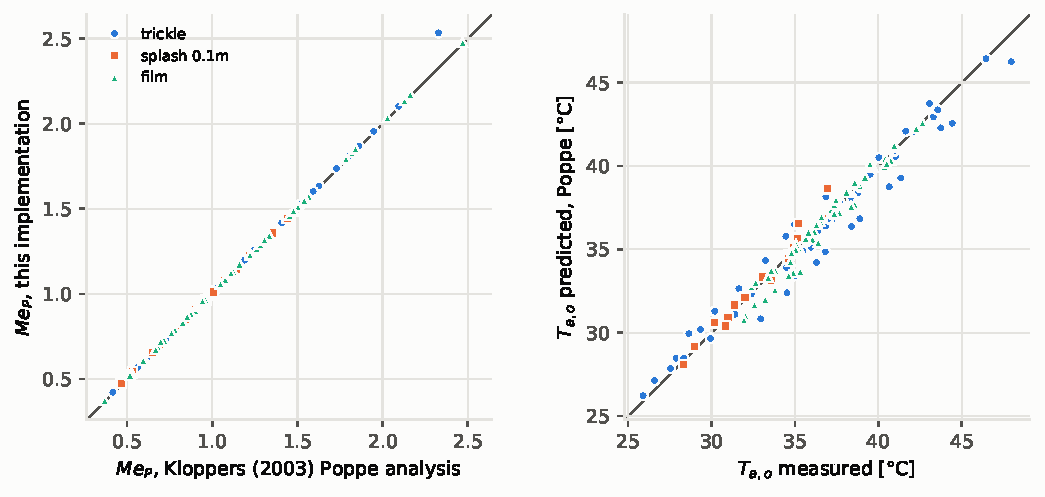
\includegraphics[width=\linewidth]{fig_kloppers_validation}
\caption{Poppe implementation against the fill tests of \citet{kloppers2003critical}. Left: Merkel number vs Kloppers'
Poppe analysis of the same tests. Right: predicted vs measured outlet-air temperature.}\label{fig:kloppers}
\end{figure}

\begin{table}[t]\centering\small
\caption{Code verification.}\label{tab:verification}
\begin{tabular}{lr}\toprule
Check & Max.\ deviation \\\midrule
Psychrometrics vs PsychroLib ($p_{ws}$, $\omega_s$, $i$, $T_{wb}$) & 0.2\,\% / 0.02\,K \\
Latent heat vs IAPWS-95 & 0.3\,\% \\
Poppe vs independent BVP, 7 cases incl.\ supersaturated near-pinch: evaporation & 0.008\,\% \\
\hspace{1em} $Me_P$ (40 steps) & 0.003\,\% \\
Poppe energy closure, unsaturated and supersaturated & $<0.1$\,\% \\
Rating mode, same fill: Merkel / Poppe / e-NTU outlet temperature & $<0.5$\,K \\
EPSAT replica vs EnergyPlus output, annual, all 14 sites & 0.2\,\% \\
Poppe fixed-point iteration, timesteps at the iteration limit: evaporation & $<10^{-3}$\,\% \\\bottomrule
\end{tabular}
\end{table}

%======================================================================
\section{Where do simplified models depart from Poppe? A climate-general map}\label{sec:map}
%======================================================================
A counterflow tower was sized with the Poppe model for a \SI{3.9}{K} approach and \SI{5.6}{K} range at
\SI{35}{\celsius}/\SI{25.6}{\celsius} design conditions and $L/G=1.2$ ($Me_P = 1.27$). With fill, $L/G$ and range fixed,
the cold-water temperature was solved with Poppe over a grid of dry-bulb ($-5$ to \SI{46}{\celsius}) and relative
humidity (5--100\,\%, wet-bulb below \SI{32}{\celsius}), and all models were evaluated at each point (Fig.~\ref{fig:map}).

\begin{figure}[t]\centering
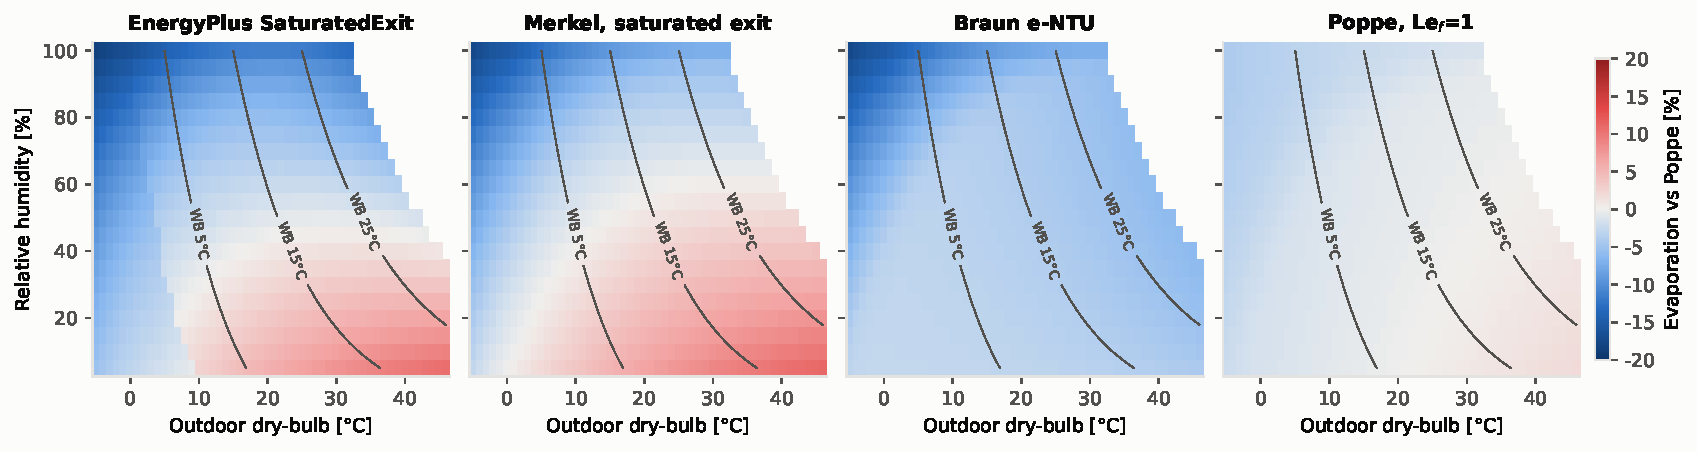
\includegraphics[width=\linewidth]{fig_method_map_physical}
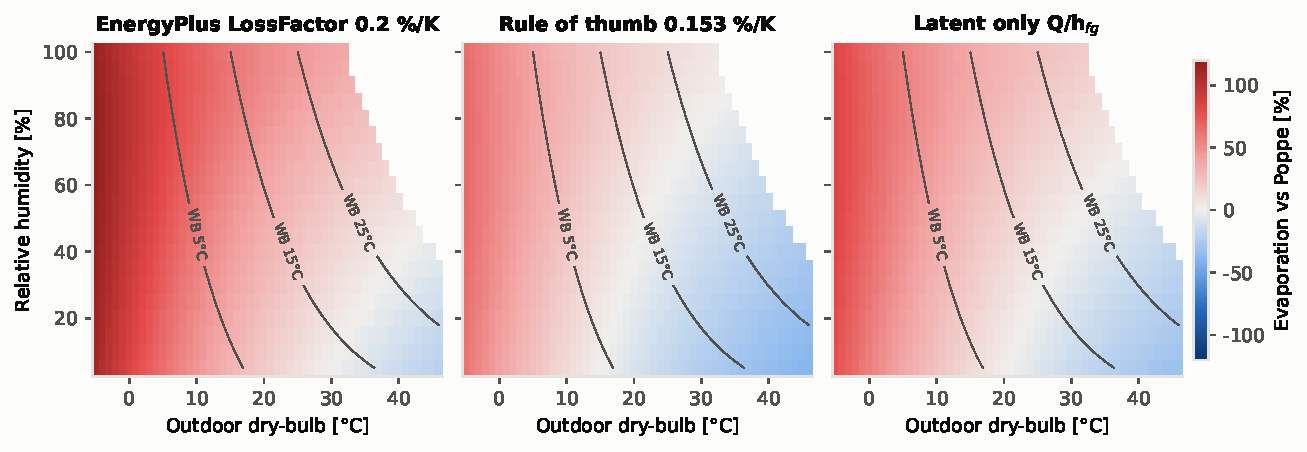
\includegraphics[width=0.8\linewidth]{fig_method_map_empirical}
\caption{Evaporation of each model relative to Poppe for a fixed tower at full load (top: $\pm$20\,\% scale; bottom:
$\pm$120\,\%). Lines: outdoor wet-bulb. Blank: wet-bulb above 32\,\textdegree C (not simulated). The step in the EnergyPlus
panel follows the 0\,\textdegree C wet-bulb line, where EnergyPlus switches its saturation-pressure formula from ice to water.}\label{fig:map}
\end{figure}

Saturated-exit models differ from Poppe by $-$19 to +11\,\% (EnergyPlus' formulation $-$18.5 to +10.5\,\%, Merkel
$-$17.5 to +11.0\,\%): they give more evaporation in hot--dry air, where the
Poppe exit air is unsaturated, and less in cold--humid air, where Poppe predicts supersaturated exhaust. The Braun model
gives 2.8--6.2\,\% less than Poppe where it can represent the exit state, and down to $-$18\,\% where it is limited to
saturated exit. The Lewis factor alone changes evaporation by $-$4.2 to +1.8\,\%. Empirical models range from $-$39 to
+117\,\%: the documented loss factor overpredicts most in cold weather, and the latent-only estimate ranges from $-$32\,\%
in hot--dry air, where sensible heat flows from the air into the water, to +84\,\% in cold air.

%======================================================================
\section{Case study: a water-cooled data center}\label{sec:case}
%======================================================================
The host model (Table~\ref{tab:dcmodel}) is a single-storey facility with two 500\,m$^2$ data halls and 1.0\,MW of
air-cooled IT equipment at 70--90\,\% CPU utilisation (mean 861\,kW, 7,540\,MWh/yr), recirculating CRAH-type air
handlers supplying 20\,\textdegree C air, three 50\,\% water-cooled variable-speed centrifugal chillers (N+1, 10\,\textdegree C
chilled water) and a three-cell \texttt{CoolingTower:VariableSpeed:Merkel} sized for a 3.9\,K approach and 5.6\,K range at
the site's 0.4\,\% evaporation design wet-bulb. Condenser water follows outdoor wet-bulb plus 3.9\,K between 18 and
29.4\,\textdegree C; the 18\,\textdegree C floor protects the chillers' minimum condenser temperature. Because the condenser loop
is sized for all three chillers, the tower is 1.5 times the duty flow, and it rejects heat in every hour (it never idles
or enters free convection). A water-side economizer, common in such plants \citep{li2020model}, was not included. Design
days, site data and tower design conditions are replaced with each site's ASHRAE values. Weather is TMYx 2011--2025 for
14 sites in ASHRAE climate zones 0A to 6A (zones from the weather files' design conditions, ASHRAE 169-2021). Annual PUE
is 1.24--1.28 and there are no unmet zone hours. EnergyPlus 22.2.0 (build c249759bad) was used.

\begin{table}[t]\centering\small
\caption{Data center model (key parameters; sources and assumptions in the supplementary model documentation).}\label{tab:dcmodel}
\begin{tabular}{ll}\toprule
IT load & 1.0\,MW design, 0.70--0.90 utilisation, UPS 95\,\% \\
Air side & 2 CRAH loops, chilled-water coils, VAV fans, 20\,\textdegree C supply, no economizer \\
Chillers & 3 $\times$ 50\,\% water-cooled VSD centrifugal, 10\,\textdegree C CHW, 6\,K design $\Delta T$ \\
Tower & Merkel VS, 3 cells (MaximalCell), approach 3.9\,K, range 5.6\,K at 0.4\,\% WB \\
Condenser control & $T_{wb}$ + 3.9\,K, limits 18--29.4\,\textdegree C \\
Water & drift 0.001\,\%; 4 cycles (headline results) \\
Weather & TMYx 2011--2025, 14 sites, climate-specific design days \\\bottomrule
\end{tabular}
\end{table}

%======================================================================
\section{Results}\label{sec:results}
%======================================================================
\subsection{Annual evaporation by model and climate}
Table~\ref{tab:sites} and Fig.~\ref{fig:dcdev} summarise the annual results. The EPSAT replica reproduces EnergyPlus'
own annual evaporation within 0.2\,\% at every site. Evaporation per unit heat rejected (Poppe) ranges from
1.05\,L/kWh$_{th}$ (Dublin, Stockholm) to 1.65\,L/kWh$_{th}$ (Riyadh), against about 1.48\,L/kWh$_{th}$ if all heat left
as latent heat. The EnergyPlus default gives less annual evaporation than Poppe at all 14 sites, by 3.7\,\% (Phoenix) to
9.3\,\% (Montreal, Stockholm). The other saturated-exit and e-NTU formulations behave similarly ($-$2.2 to $-$7.3\,\%), and
the Lewis factor alone accounts for 0.1--2.1\,\%. Unlike the full-load map, saturated-exit models do not give more
evaporation than Poppe in hot--dry climates here, not even in hours above 30\,\textdegree C ($-$3.4\,\% at Phoenix). The
reason is the operating point rather than the climate: with the N+1 condenser flow and a 3.9\,K approach, this tower runs
at a median $L/G$ of 1.6--1.9 at the hot--dry sites, with exit air close to saturation, whereas the map
tower runs at $L/G=1.2$. At 40\,\textdegree C and 21\,\textdegree C wet-bulb with this approach and range, the EnergyPlus formula gives
2\,\% more evaporation than Poppe at $L/G=1.2$ but 5\,\% less at $L/G=1.64$. Section~\ref{sec:consistency} tests this with
an ordinary fill.

\begin{figure}[t]\centering
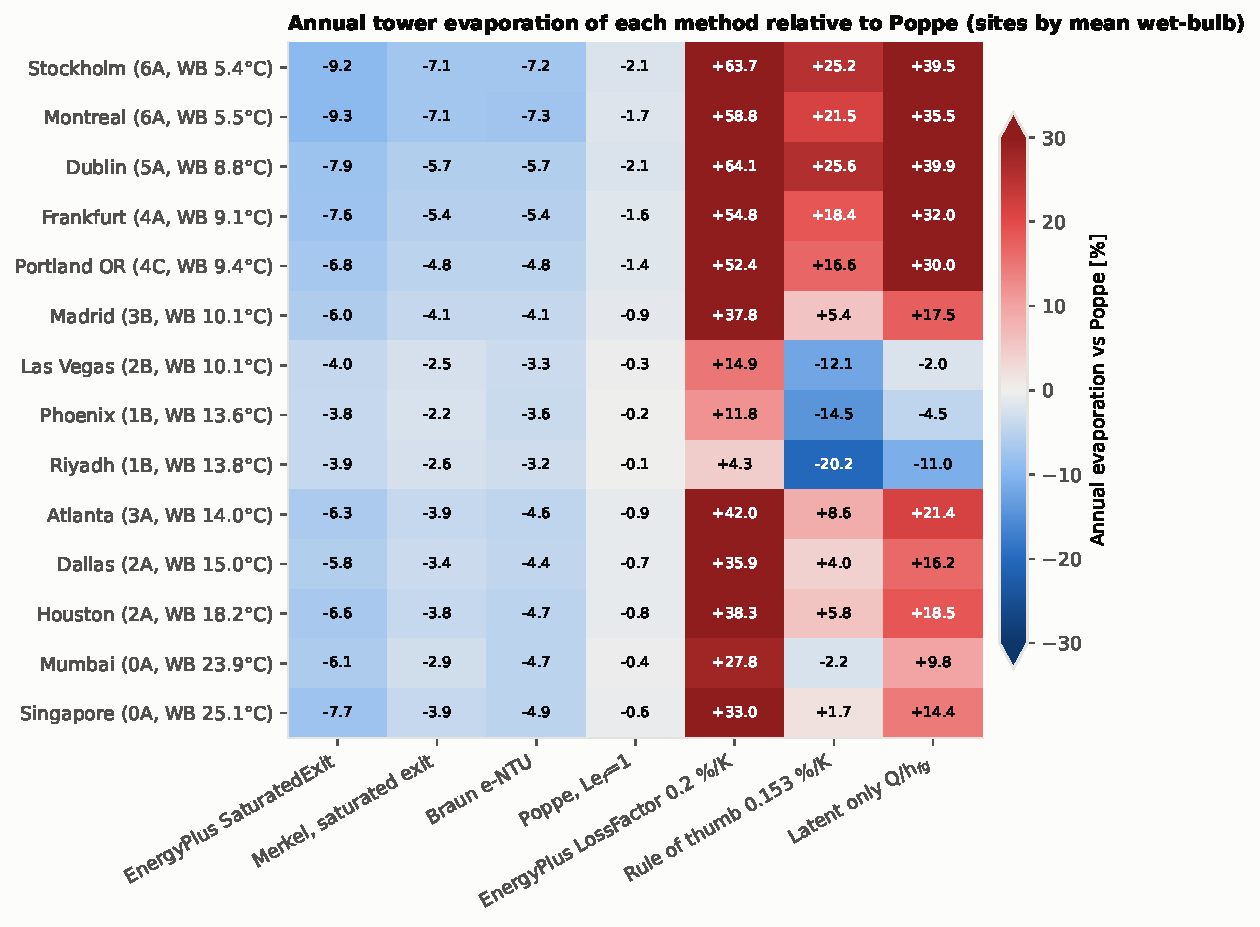
\includegraphics[width=\linewidth]{fig_dc_method_deviation}
\caption{Annual evaporation of each model relative to Poppe (vapour and mist) for the data center in 14 climates, sites
sorted by mean wet-bulb. The colour scale is limited to $\pm$30\,\%; values are printed in each cell.}\label{fig:dcdev}
\end{figure}

\begin{table}[t]\centering\scriptsize
\caption{Annual results by site (sorted by mean wet-bulb). $E_P$: Poppe evaporation including mist; mist: liquid share of
$E_P$; EP SatExit vs Poppe for total and vapour-only Poppe evaporation; corr.: share of hours with the near-pinch air-flow
correction; LF: documented loss factor (0.2\,\%/K) vs Poppe.}\label{tab:sites}
\resizebox{\linewidth}{!}{\begin{tabular}{llrrrrrrrrrr}
\toprule
Site & CZ & $\bar T_{wb}$ & PUE & $Q$ & $E_{P}$ & mist & $E_P/Q$ & \multicolumn{2}{c}{EP SatExit vs Poppe [\%]} & corr. & LF \\
 & & [\textdegree C] & & [MWh] & [m$^3$] & [\%] & [L/kWh$_{th}$] & total & vapour & [\% h] & [\%] \\
\midrule
Stockholm & 6A & 5.4 & 1.24 & 9254 & 9755 & 4.9 & 1.05 & -9.3 & -4.6 & 100 & +64 \\
Montreal & 6A & 5.5 & 1.25 & 9282 & 10086 & 4.8 & 1.09 & -9.3 & -4.8 & 0 & +59 \\
Dublin & 5A & 8.8 & 1.24 & 9264 & 9741 & 3.5 & 1.05 & -7.9 & -4.6 & 99 & +64 \\
Frankfurt & 4A & 9.1 & 1.25 & 9281 & 10348 & 3.1 & 1.11 & -7.6 & -4.6 & 66 & +55 \\
Portland OR & 4C & 9.4 & 1.24 & 9277 & 10502 & 2.5 & 1.13 & -6.8 & -4.5 & 95 & +52 \\
Madrid & 3B & 10.1 & 1.25 & 9314 & 11661 & 1.7 & 1.25 & -6.0 & -4.4 & 66 & +38 \\
Las Vegas & 2B & 10.1 & 1.25 & 9344 & 14039 & 0.3 & 1.50 & -4.0 & -3.7 & 0 & +15 \\
Phoenix & 1B & 13.6 & 1.25 & 9368 & 14456 & 0.2 & 1.54 & -3.7 & -3.5 & 0 & +12 \\
Riyadh & 1B & 13.8 & 1.25 & 9363 & 15485 & 0.1 & 1.65 & -3.9 & -3.8 & 0 & +4 \\
Atlanta & 3A & 14.0 & 1.26 & 9374 & 11394 & 1.3 & 1.22 & -6.3 & -5.1 & 0 & +42 \\
Dallas & 2A & 15.0 & 1.26 & 9388 & 11922 & 1.0 & 1.27 & -5.8 & -4.8 & 0 & +36 \\
Houston & 2A & 18.2 & 1.27 & 9438 & 11775 & 1.0 & 1.25 & -6.7 & -5.7 & 0 & +38 \\
Mumbai & 0A & 23.9 & 1.28 & 9559 & 12904 & 0.1 & 1.35 & -6.3 & -6.2 & 0 & +28 \\
Singapore & 0A & 25.1 & 1.28 & 9592 & 12448 & 0.3 & 1.30 & -7.9 & -7.6 & 0 & +33 \\
\bottomrule
\end{tabular}
}
\end{table}

\subsection{Vapour and liquid mist}\label{sec:mist}
In cold and mild climates Poppe predicts supersaturated exhaust in many hours (exit air carrying more than 0.1\,g/kg of
liquid in 400\,h/yr in Mumbai to 7,200\,h/yr in Dublin). The liquid share of Poppe evaporation is below 0.4\,\% in Phoenix, Riyadh, Las Vegas, Mumbai
and Singapore, 1.0--2.5\,\% in Atlanta, Dallas, Houston, Madrid and Portland, and 3.1--4.9\,\% in Frankfurt, Dublin,
Montreal and Stockholm, where it accounts for about half of the difference
from EnergyPlus. Whether this mist is consumed depends on how much of it the drift eliminators capture and return to the
basin; vapour-only Poppe evaporation is therefore a lower bound and total evaporation an upper bound. Against vapour-only
Poppe the EnergyPlus default gives 3.5\,\% (Phoenix) to 7.6\,\% (Singapore) less evaporation.

\subsection{Dependence on the tower's thermal operating point}\label{sec:consistency}
Accounting mode evaluates every model at EnergyPlus' air flow, so the results depend on how EnergyPlus sizes and operates
the tower. The base tower is autosized for a 3.9\,K approach at each site's 0.4\,\% design wet-bulb with N+1 water flow
(design $L/G$ 1.6--1.8). Where the design wet-bulb is 21\,\textdegree C or lower (Dublin, Frankfurt, Madrid, Portland,
Stockholm) this design point is itself close to the pinch, with design Merkel numbers of 5.4--7.6 against 1.5--3.3
elsewhere (Table~\ref{tab:fill}). At these five sites the near-pinch correction (Section~\ref{sec:airflow}) was needed in
66--100\,\% of hours, with a mean air-flow factor of 1.02--1.03 (maximum 1.05); elsewhere it was needed in fewer than
0.3\,\% of hours. The correction therefore follows the design wet-bulb, not the winter climate: Montreal, as cold as
Stockholm but with a 23.5\,\textdegree C design wet-bulb, needs none and has the same EnergyPlus--Poppe difference
($-$9.3\,\%). The equipment-informed plant (Section~\ref{sec:sensitivity}) needs no correction at any site. Near the
pinch the implied $Me_P$ becomes very large (median 1.6--6.2 by site, maximum 78).

Two checks quantify the dependence. First, Poppe was solved in rating mode for a \emph{fixed} fill sized at EnergyPlus'
design point (with the same minimal air correction where needed, 3\,\% at Stockholm) and scaled off-design as
$Me_P\propto(L/G)^{-n}$ with $n=0.6$ (and 0.5 and 0.78, Section~\ref{sec:sensitivity}). For every loaded hour at Phoenix,
Singapore, Frankfurt and Stockholm, at EnergyPlus' inlet water temperature, water flow, air flow and weather, the
fixed-fill cold-water temperature differs from EnergyPlus' by $-$0.09 to +0.11\,K (median), heat rejected by $-$2.4 to
+2.5\,\%, evaporation by $-$2.3 to +2.5\,\% and evaporation per unit heat by at most 0.17\,\%. Per unit heat is the
relevant measure for the model comparison, because accounting mode imposes EnergyPlus' heat rejection on every model. This
fill, however, inherits EnergyPlus' near-pinch design ($Me_P$ of 6.5 and 7.6 at Frankfurt and Stockholm) and does not
represent an ordinary tower.

Second, the EnergyPlus tower was replaced by one with an ordinary fill: a design $L/G$ of 1.0, 1.2 or 1.4 (design $Me_P$
1.0--2.7) at the same design water flow and conditions, with $Me_P\propto(L/G)^{-0.6}$. For every loaded hour the air flow
this tower needs to deliver EnergyPlus' leaving-water temperature was solved, so heat rejected is unchanged and only the air
flow differs. Hours in which even the design air flow cannot reach that temperature are excluded (up to 14\,\% at Houston
and Mumbai, where the ordinary tower is smaller than EnergyPlus'). The ordinary tower runs with 11--45\,\% more air
(median, design $L/G$ 1.2), and its Poppe evaporation differs from the accounting-mode value by $-$0.1 to +6.4\,\%, most at
hot--dry sites. At its operating point the EnergyPlus SaturatedExit formula differs from Poppe by $-$9.1 to $-$3.4\,\% at
Stockholm, Montreal, Dublin, Frankfurt and Portland, by $-$6.0 to +3.0\,\% at Madrid and the warm--humid sites, and by
$-$2.0 to +10.9\,\% at Phoenix, Las Vegas and Riyadh, where the sign depends on the design $L/G$ (Table~\ref{tab:fill}).
The shortfall of the EnergyPlus default in cold and mild climates is therefore robust to the tower model. In hot--dry
climates EnergyPlus can under- or overestimate evaporation, consistent with the full-load map, and the sign depends on the
tower's air-to-water ratio.

\begin{table}[t]\centering\scriptsize
\caption{Design point of the EnergyPlus tower and the ordinary-fill check (sites sorted by mean wet-bulb). $T_{wb,d}$:
design wet-bulb; $Me_{P,d}$: Poppe Merkel number at the design point; corr.: share of loaded hours with the near-pinch
air-flow correction; EP vs P: EnergyPlus SaturatedExit vs Poppe annual evaporation. Ordinary fill: design $L/G$ = 1.2, and
range over design $L/G$ = 1.0--1.4; P shift: Poppe evaporation with the ordinary fill vs accounting mode; capped: hours
excluded because the ordinary tower cannot reach EnergyPlus' leaving-water temperature.}\label{tab:fill}
\resizebox{\linewidth}{!}{\begin{tabular}{lrrrrrrrrr}
\toprule
 & \multicolumn{4}{c}{EnergyPlus tower (base plant)} & \multicolumn{5}{c}{Ordinary fill, design $L/G$ = 1.0--1.4} \\
\cmidrule(lr){2-5}\cmidrule(lr){6-10}
Site & $T_{wb,d}$ & $Me_{P,d}$ & corr. & EP vs P & $Me_{P,d}$ & EP vs P & EP vs P & P shift & capped \\
 & [\textdegree C] & & [\% h] & [\%] & ($L/G$=1.2) & ($L/G$=1.2) [\%] & range [\%] & [\%] & [\% h] \\
\midrule
Stockholm & 20.0 & 7.6 & 100 & -9.3 & 2.05 & -8.9 & -9.1 to -8.5 & +0.3 & 0.0 \\
Montreal & 23.5 & 2.8 & 0 & -9.3 & 1.51 & -7.9 & -8.6 to -6.6 & +0.5 & 0.1 \\
Dublin & 20.0 & 7.2 & 99 & -7.9 & 2.07 & -7.7 & -7.8 to -7.3 & -0.0 & 0.0 \\
Frankfurt & 21.0 & 6.5 & 66 & -7.6 & 1.85 & -6.5 & -7.2 to -5.1 & +1.0 & 0.0 \\
Portland OR & 20.8 & 7.2 & 95 & -6.8 & 1.87 & -5.3 & -6.2 to -3.4 & +1.5 & 0.0 \\
Madrid & 20.0 & 5.4 & 66 & -6.0 & 2.01 & -4.0 & -5.4 to -1.3 & +2.4 & 0.0 \\
Las Vegas & 22.5 & 2.7 & 0 & -4.0 & 1.60 & +1.5 & -2.0 to +7.1 & +3.2 & 0.0 \\
Phoenix & 24.1 & 2.4 & 0 & -3.7 & 1.42 & +4.0 & -0.4 to +10.9 & +3.4 & 0.3 \\
Riyadh & 21.8 & 3.3 & 0 & -3.9 & 1.69 & +2.5 & -1.6 to +9.5 & +4.9 & 0.0 \\
Atlanta & 25.1 & 2.0 & 0 & -6.3 & 1.33 & -3.4 & -5.0 to -0.7 & +1.1 & 2.7 \\
Dallas & 25.8 & 2.0 & 0 & -5.8 & 1.26 & -1.6 & -3.9 to +2.0 & +1.5 & 8.5 \\
Houston & 26.8 & 1.8 & 0 & -6.7 & 1.17 & -3.2 & -5.1 to -0.3 & +1.1 & 13.1 \\
Mumbai & 28.4 & 1.5 & 0 & -6.3 & 1.05 & -0.9 & -3.5 to +3.0 & +1.4 & 13.8 \\
Singapore & 28.0 & 1.6 & 0 & -7.9 & 1.08 & -4.4 & -6.0 to -1.8 & +1.0 & 1.7 \\
\bottomrule
\end{tabular}
}
\end{table}

\subsection{Peak day and seasonal pattern}
On each site's peak evaporation day the EnergyPlus default gives 1.2--7.2\,\% less evaporation than Poppe. At the
timestep level the largest differences, $-$15 to $-$29\,\%, occur below 0\,\textdegree C, where Poppe exhaust is
supersaturated (Fig.~\ref{fig:dcts}). Empirical
models do not follow the climate signal (Fig.~\ref{fig:dcmonthly}): the documented loss factor is nearly constant through
the year.

\begin{figure}[t]\centering
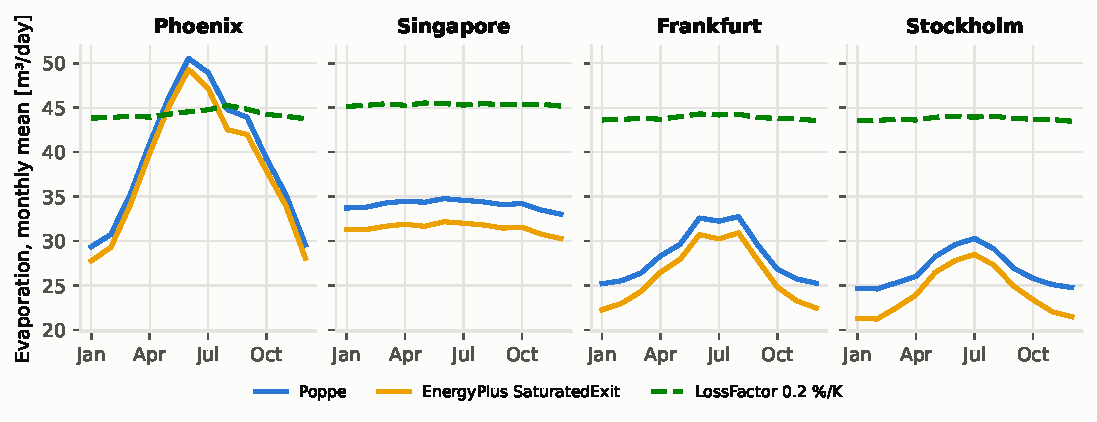
\includegraphics[width=\linewidth]{fig_dc_monthly}
\caption{Monthly mean daily evaporation: Poppe, EnergyPlus SaturatedExit and LossFactor (0.2\,\%/K as documented).}\label{fig:dcmonthly}
\end{figure}

\begin{figure}[t]\centering
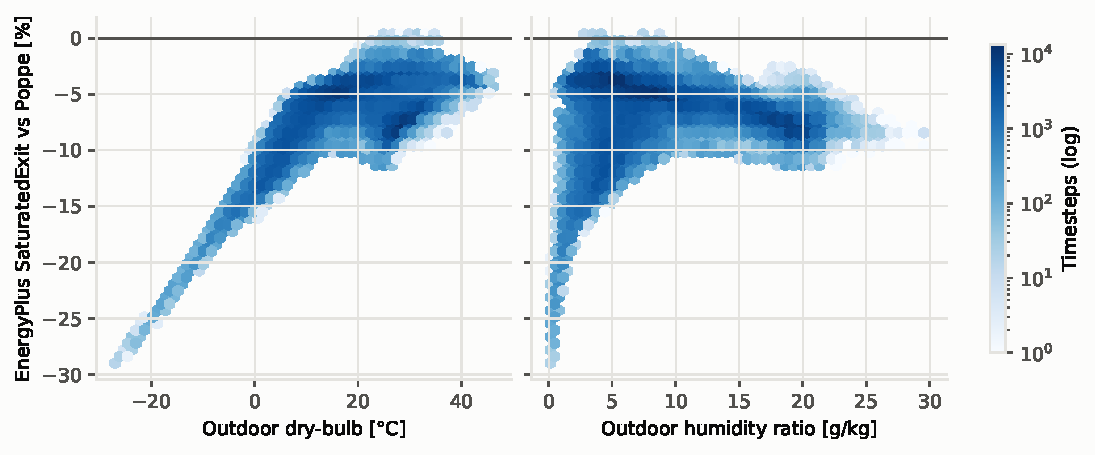
\includegraphics[width=\linewidth]{fig_dc_timestep_deviation}
\caption{Timestep difference of EnergyPlus SaturatedExit from Poppe (vapour and mist) against outdoor dry-bulb and humidity
ratio, all 14 sites. The largest differences ($-$15 to $-$29\,\%) occur below 0\,\textdegree C, where Poppe exhaust is
supersaturated.}\label{fig:dcts}
\end{figure}

\subsection{Sensitivity}\label{sec:sensitivity}
Table~\ref{tab:sens} shows that the EnergyPlus--Poppe difference changes by up to 1.1 percentage points when the
tower is sized for duty instead of N+1 or the condenser floor is lowered to 15\,\textdegree C (four sites). An equipment-informed plant,
built from the specifications of chillers and towers common in data centers (supplementary \texttt{docs/EQUIPMENT\_SPECS.md}),
was run at all 14 sites. It uses 15.5\,\textdegree C chilled water, the ASHRAE 90.1 Set S centrifugal-chiller curves
\citep{ashrae2019addendumbd}, a 15.5\,\textdegree C condenser floor, UA modifiers fitted to the fill data of
\citet{kloppers2003critical} ($UA\propto AFR^{0.7}\,WFR^{0.58}$), a 0.25 minimum fan speed and 50\,\% cell turndown. Its
difference from Poppe is $-$8.4 to $-$2.5\,\%, 0.4--1.2 points smaller than the base plant at every site, which is 5\,\%
of the base result at Singapore and a third of it at Phoenix ($-$3.7 to $-$2.5\,\%); PUE stays at 1.24--1.28. Plant
variants therefore preserve the sign of the difference and its ranking across sites; replacing the tower by one with an
ordinary fill does not at hot--dry sites (last row of Table~\ref{tab:sens}). In the fixed-fill check
(Section~\ref{sec:consistency}), fill exponents of 0.5, 0.6 and 0.78 change evaporation per unit heat by at most
0.17\,\%; 0.78 is the air-flow exponent of Kloppers' published film-fill correlation and bounds the $L/G$ exponents of
0.51--0.60 fitted in Section~\ref{sec:verification} from above. Over the documented loss-factor
range (0.15--0.27\,\%/K) the loss-factor estimate spans $-$22 to +122\,\% of Poppe across sites. The Lewis factor changes
evaporation by 0.1--2.1\,\% (POPPE vs POPPE1). Drift (0.001\,\%) is below 0.2\,\% of makeup in all cases. Weather-year
variability was not studied; a single typical year per site was used.

\begin{table}[t]\centering\small
\caption{EnergyPlus SaturatedExit vs Poppe annual evaporation [\%] for plant variants. $^a$15.5\,\textdegree C chilled water
and condenser floor, ASHRAE 90.1 Set S chiller curves, fill-data UA curves, 0.25 minimum fan speed, 50\,\% cell turndown. $^b$Same EnergyPlus runs as the base plant, tower replaced by an ordinary fill
(Section~\ref{sec:consistency}); hours the ordinary tower cannot meet are excluded. Variants with ``--'' were run only at
the four sites shown.}\label{tab:sens}
\begin{tabular}{lrrrrr}
\toprule
Plant variant & Phoenix & Singapore & Frankfurt & Stockholm & All sites ($n$) \\
\midrule
Base (N+1 tower, 18\,\textdegree C floor) & -3.7 & -7.9 & -7.6 & -9.3 & -9.3 to -3.7 (14) \\
Tower sized for duty (2 chillers) & -4.4 & -8.4 & -7.7 & -9.3 & -- \\
Condenser floor 15\,\textdegree C & -3.1 & -7.9 & -6.6 & -8.2 & -- \\
Both & -4.1 & -8.4 & -6.9 & -8.4 & -- \\
Equipment-informed plant$^a$ & -2.5 & -7.5 & -6.7 & -8.3 & -8.4 to -2.5 (14) \\
\bottomrule
\end{tabular}

\end{table}

\subsection{Water usage effectiveness and makeup-water quality}\label{sec:wue}
With EnergyPlus' four cycles, the EnergyPlus default gives a WUE 3.7--9.3\,\% below the Poppe value (1.56--2.63
against 1.72--2.74\,L/kWh$_{IT}$ across sites; Fig.~\ref{fig:wue}). With each site's own makeup water, the allowable
cycles and hence blowdown differ widely between sites (Table~\ref{tab:waterquality}). Soft supplies (Atlanta, Portland,
Madrid, Singapore, Dublin, Stockholm) reach 5.7--10 cycles. At Atlanta, Portland and Madrid every limit set gives the
model's 10-cycle cap ($-$17\,\%), at Portland and Madrid partly because sulfate, chloride or silica data are missing, so
these results reflect the cap rather than the chemistry. Supplies with moderate alkalinity (Dallas, Houston, Montreal,
Mumbai) are limited by alkalinity unless acid is fed ($-$14 to +3\,\% without capped cases). Frankfurt's hard water allows
2.3--4.7 cycles ($-$5 to +31\,\%) and Riyadh's chloride 2.1--4.1 cycles ($-$1 to +44\,\%). Colorado River water at Phoenix
and Las Vegas already carries 210--240\,mg/L sulfate, so the 250\,mg/L sulfate limits of two galvanized-steel sets allow
about one cycle, which the model raises to its 1.5-cycle floor (+125\,\%). This does not describe credible operation:
such sites use stainless steel, acid feed or side-stream treatment, and the other three sets give 2.5--3.3 cycles (+7 to
+25\,\%). Excluding cases at the cap or floor, site water changes makeup by $-$16 to +44\,\% relative to four cycles.
The cycles of concentration are an operating set-point rather than a modelling choice, and their effect multiplies that of
the evaporation model, which changes makeup by 3.7--9.3\,\% at any fixed cycles. Simulated WUE is therefore at least as
sensitive to the assumed cycles as to the evaporation model, and site cycles, or the water quality and treatment program
behind them, should be reported with any simulated WUE. Two caveats apply. Soft, low-alkalinity waters are in practice
limited by corrosion, which the model does not represent, so their high-cycle results are optimistic. Data confidence is
low for Atlanta, Madrid and Mumbai and low to medium for Dallas, where no treated-water mineral data were found.

\begin{table}[t]\centering\scriptsize
\caption{Site makeup water and cycles of concentration. Data: confidence of the water-quality data (H high, M medium,
L low); $^\dagger$sulfate, chloride or silica missing (treated as non-limiting). $N_{c,\mathrm{eff}}$: effective annual
cycles $E/(B+D_r)+1$, range over the five limit sets. $\Delta$WUE: Poppe makeup per IT energy relative to fixed four
cycles, over all sets ($^c$lower end at the 10-cycle cap; $^f$upper end at the 1.5-cycle floor) and over the sets at
neither bound (``--'': none). ``min.'': raised to the 1.5-cycle minimum.}\label{tab:waterquality}
\begin{tabular}{lrrrrlrlrrr}
\toprule
Site & Ca & Alk. & SO$_4$ & Cl & Data & $N_{c,\mathrm{eff}}$ & Limit (lowest $N_c$) & WUE$_{N=4}$ & $\Delta$WUE, all sets & $\Delta$WUE, unclamped \\
 & \multicolumn{4}{c}{[mg/L; Ca, Alk.\ as CaCO$_3$]} & & & & [L/kWh] & [\%] & [\%] \\
\midrule
Stockholm & 65 & 45 & 44 & 16 & M--H$^\dagger$ & 5.7--10.0 & sulfate & 1.73 & -17$^c$ to -9 & -16 to -9 \\
Montreal & 77 & 93 & 22 & 26 & H & 4.3--10.0 & alkalinity & 1.78 & -17$^c$ to -2 & -11 to -2 \\
Dublin & 47 & 28 & 35 & 25 & M$^\dagger$ & 7.1--10.0 & sulfate & 1.72 & -17$^c$ to -13 & -13 to -13 \\
Frankfurt & 170 & 171 & 45 & 22 & M & 2.3--4.7 & alkalinity & 1.83 & -5 to +31 & -5 to +31 \\
Portland OR & 5 & 29 & -- & -- & H$^\dagger$ & 10.0--10.0 & cap (10) & 1.86 & -17$^c$ to -17 & -- \\
Madrid & 40 & 40 & -- & -- & L$^\dagger$ & 10.0--10.0 & cap (10) & 2.06 & -17$^c$ to -17 & -- \\
Las Vegas & 187 & 112 & 209 & 99 & H & 1.5--3.2 & sulfate (min.) & 2.48 & +9 to +125$^f$ & +9 to +21 \\
Phoenix & 188 & 132 & 239 & 90 & M--H & 1.5--3.3 & sulfate (min.) & 2.56 & +7 to +125$^f$ & +7 to +25 \\
Riyadh & 146 & 80 & 88 & 120 & M$^\dagger$ & 2.1--4.1 & chloride & 2.74 & -1 to +44 & -1 to +44 \\
Atlanta & 8 & 12 & 4 & 3 & L & 10.0--10.0 & cap (10) & 2.01 & -17$^c$ to -17 & -- \\
Dallas & 105 & 110 & 33 & 20 & L--M & 3.6--7.6 & alkalinity & 2.11 & -14 to +3 & -14 to +3 \\
Houston & 97 & 95 & 21 & 38 & M & 4.2--7.8 & alkalinity & 2.08 & -14 to -2 & -14 to -2 \\
Mumbai & 35 & 97 & -- & 10 & L$^\dagger$ & 4.1--10.0 & alkalinity & 2.28 & -17$^c$ to -1 & -10 to -1 \\
Singapore & 39 & 35 & 7 & 30 & H & 8.3--10.0 & chloride & 2.20 & -17$^c$ to -15 & -15 to -15 \\
\bottomrule
\end{tabular}

\end{table}

\begin{figure}[t]\centering
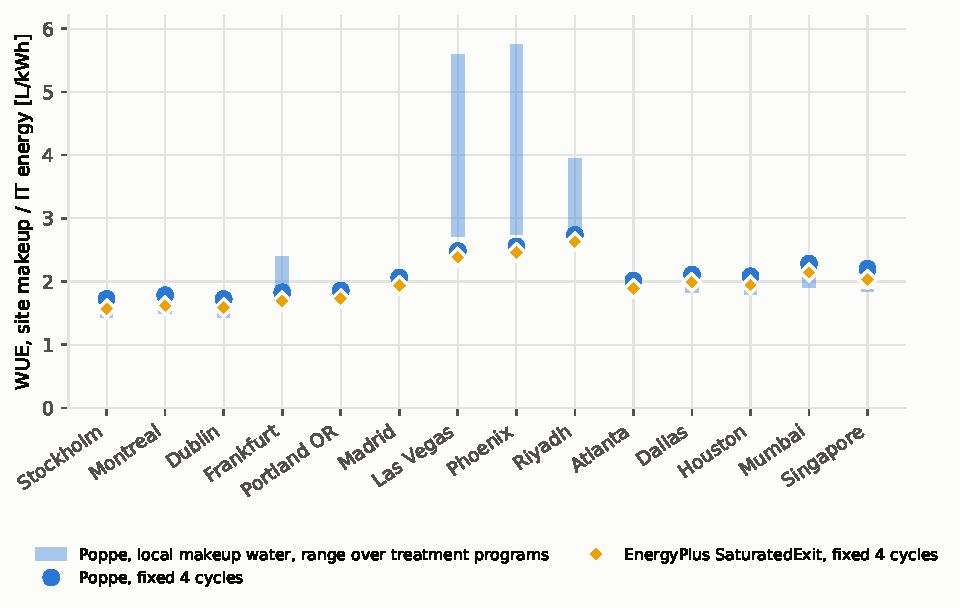
\includegraphics[width=\linewidth]{fig_dc_water_quality}
\caption{WUE by climate. Diamonds: EnergyPlus default (SaturatedExit, 4 cycles). Circles: Poppe evaporation, 4 cycles.
Bars: Poppe evaporation with each site's makeup water, range over five treatment limit sets; ``cap'' and ``floor''
mark range ends set by the model's 10-cycle cap or 1.5-cycle floor.}\label{fig:wue}
\end{figure}

%======================================================================
\section{The EnergyPlus loss-factor input}\label{sec:lossfactor}
%======================================================================
The EnergyPlus input dictionary documents the evaporation loss factor in percent per kelvin (default 0.2, typical
0.15--0.27), but \texttt{CondenserLoopTowers.cc} (v22.2.0 and the development branch in October 2026) uses the input
without dividing by 100, while the drift percentage read alongside it is divided by 100. A run of the stock
\texttt{CoolingTower\_VariableSpeed.idf} with the documented default gives an implied factor of 0.2001\,K$^{-1}$, i.e.\
20\,\%/K, with evaporation reaching 24\,\% of the circulating water. Users who adopt the documented values therefore
overestimate evaporation by two orders of magnitude. All LF results in this paper use the documented intent (0.2\,\%/K).
Other water-accounting issues found during this work, with their evidence status, are listed in Appendix~\ref{app:issues};
they did not affect the case study.

%======================================================================
\section{Discussion}
%======================================================================
\paragraph{Interpretation} The differences reported here are between models, not errors against measurements. Poppe is
the most complete of the models considered; it is verified against an independent solution and reproduces measured
fill-test outlet-air temperatures better than saturated-exit analyses. Those tests, however, cover only mild inlet air with
supersaturated exhaust and do not measure evaporation, and no metered makeup of an operating tower was available. The results show how much a water estimate depends on the
chosen model and where that dependence is largest.

\paragraph{Which model to use} For annual totals, saturated-exit and e-NTU models are within about 10\,\% of Poppe. In
cold and mild climates they are consistently lower, by 3--9\,\% for both the EnergyPlus tower and an ordinary fill; in
hot--dry climates the sign depends on the tower's air-to-water ratio, so neither under- nor overestimation can be assumed.
At the timestep level the difference reaches $-$29\,\% in freezing weather, so hourly or peak-hour water estimates in cold
climates should use Poppe. At the documented 0.2\,\%/K the loss factor exceeds Poppe at every site (+4 to +64\,\%, more than +50\,\% at the
five coolest sites), and the rule-of-thumb and latent-only estimates change sign with climate; none of them follows the
climate signal, and they should not be used for siting or permitting. Because the mist share depends on drift
eliminators, reporting vapour-only and total Poppe evaporation as a range is recommended.

\paragraph{Limitations} (i) Accounting mode uses EnergyPlus' air flow. For the same heat and leaving-water temperature,
Poppe evaporation with an ordinary fill differs from the accounting value by up to 6.4\,\% at hot--dry sites, where the
sign of the EnergyPlus difference also changes; an EnergyPlus tower model with a Poppe thermal solution and a
characterised fill would remove this dependence. (ii) The fill tests measure outlet-air temperature, not evaporation, and
cover only mild inlet air with supersaturated exhaust; metered makeup and blowdown of an operating tower are still needed,
in particular in hot--dry and freezing conditions. (iii) One plant type and one typical weather year per site were
studied; plant variants changed the main result by 0.4--1.2 percentage points, up to a third of it at hot--dry sites.
(iv) Makeup-water data are of low confidence at four sites and incomplete at five; corrosion limits are not modelled;
cycles are assumed to follow the water temperature instantly; and the recirculating pH without acid feed is assumed.

%======================================================================
\section{Conclusions}
%======================================================================
\begin{enumerate}
\item An EnergyPlus plugin evaluates eight evaporation models on the same operating point every timestep. The Poppe
implementation agrees with an independent solution within 0.01\,\% for unsaturated and supersaturated air, and it
reproduces measured fill-test outlet-air temperatures better than saturated-exit analyses (0.84 against 1.10\,K rms).
\item For a fixed tower at full load, saturated-exit models differ from Poppe by $-$19 to +11\,\% depending on ambient
conditions, and empirical models by $-$39 to +117\,\%.
\item For a 1\,MW data center in 14 climates, the EnergyPlus default gives 3.7--9.3\,\% less annual evaporation than Poppe
(3.5--7.6\,\% excluding mist). The shortfall in cold and mild climates (3--9\,\%) is robust to plant variants and to
replacing EnergyPlus' tower by one with an ordinary fill; in hot--dry climates its magnitude and sign depend on the
tower's air-to-water ratio ($-$2 to +11\,\% with ordinary fills).
\item Over the documented loss-factor range, loss-factor estimates deviate from Poppe by $-$22 to +122\,\%.
\item With each site's own makeup water, cycles of concentration set by sourced treatment limits change makeup by $-$16
to +44\,\% relative to four cycles, and by more where the model's cycle bounds apply. The cycles assumption is at least
as important for simulated WUE as the evaporation model and multiplies its effect, so site cycles or water data should
accompany any simulated water-use estimate.
\item The EnergyPlus \texttt{LossFactor} input is applied as a fraction instead of a percentage, inflating that method's
evaporation 100-fold.
\end{enumerate}

\section*{Data and code availability}
The plugin, models, weather metadata, run archive and scripts that reproduce every figure and table are available at
\url{https://github.com/TensorBuildLab/EnergyPlus-HeatRejection-Water} under the MIT licence. \texttt{reproduce.sh} regenerates all results with EnergyPlus 22.2.0.

\appendix
\section{Other water-accounting issues in EnergyPlus heat-rejection models}\label{app:issues}
\begin{table}[h]\centering\scriptsize
\begin{tabular}{p{0.38\linewidth}p{0.55\linewidth}}\toprule
Issue & Evidence \\\midrule
Idle towers book evaporation, drift and blowdown (water use computed from a stale air-flow ratio before \texttt{report()} zeroes
the tower outputs) & Reproduced with stock files: in \texttt{CoolingTower\_VariableSpeed.idf} (Golden, annual) the second tower
rejects no heat but books 8.65\,m$^3$ in 2,823 timesteps. Not observed with the Merkel tower in the case study. \\
Merkel tower books no evaporation in free convection (air-flow ratio set to 0 while heat is rejected) & Reproduced in
the equipment-informed plant at Montreal: 4.2\,h at $-$21 to $-$27\,\textdegree C with the fans off and about 320\,kW
rejected, with zero EnergyPlus evaporation (Poppe: 1.0\,m$^3$, 0.01\,\% of the annual total). Not triggered in the base
plant, whose tower never enters free convection. \\
Regression-based variable-speed towers use the free-convection capacity fraction as an air-flow ratio & Code inspection;
observed in the stock example as ratios of 0.125--0.14 in fan-off and cycling hours. \\
Fluid-cooler air flow autosized as $\dot Q_{nom}[\mathrm W]/(T_{w,in}-T_{a,in})\times4$ read as m$^3$/s & Reproduced:
14,061\,m$^3$/s for the 58.6\,kW stock \texttt{FluidCoolerTwoSpeed.idf}, about 2,900 times a physical value at a 10\,K air
temperature rise; affects air-side quantities only. \\\bottomrule
\end{tabular}
\end{table}
None of these issues, nor the loss-factor error of Section~\ref{sec:lossfactor}, has yet been confirmed on EnergyPlus
26.2 or reported to the developers; reproductions are provided in the supplementary material (\texttt{bugreports/}), and
the issues will be filed before publication.

\bibliographystyle{elsarticle-harv}
\bibliography{references}
\end{document}
